\documentclass[../../main.tex]{subfiles}
\graphicspath{{images/Maschinentechnik/}{../../images/Maschinentechnik/}}

\begin{document}
    \subsection{Konzeptbeschreibung}
    Die Lokomotive in Abbildung \ref{fig:bg_lokomotive} in die drei Unterbaugruppen Antriebswagen (Position 1), Führungswagen (Position 2) und Ladungsträger (Position 3) unterteilt. Der Antriebswagen enthält alle notwendigen Komponenten, um die Lokomotive zu beschleunigen und wieder abzubremsen. Zusätzlich sind die Kameras für die Spur- und Signalerkennung an ihm angebracht. Der Führungswagen hingegen dient lediglich als Abstützung für den Ladungsträger. Er bietet aber zusätzlichen Bauraum für elektronische Komponenten.\\

    \begin{figure}[H] %Lokomotive mit Positionsnummern
        \centering
        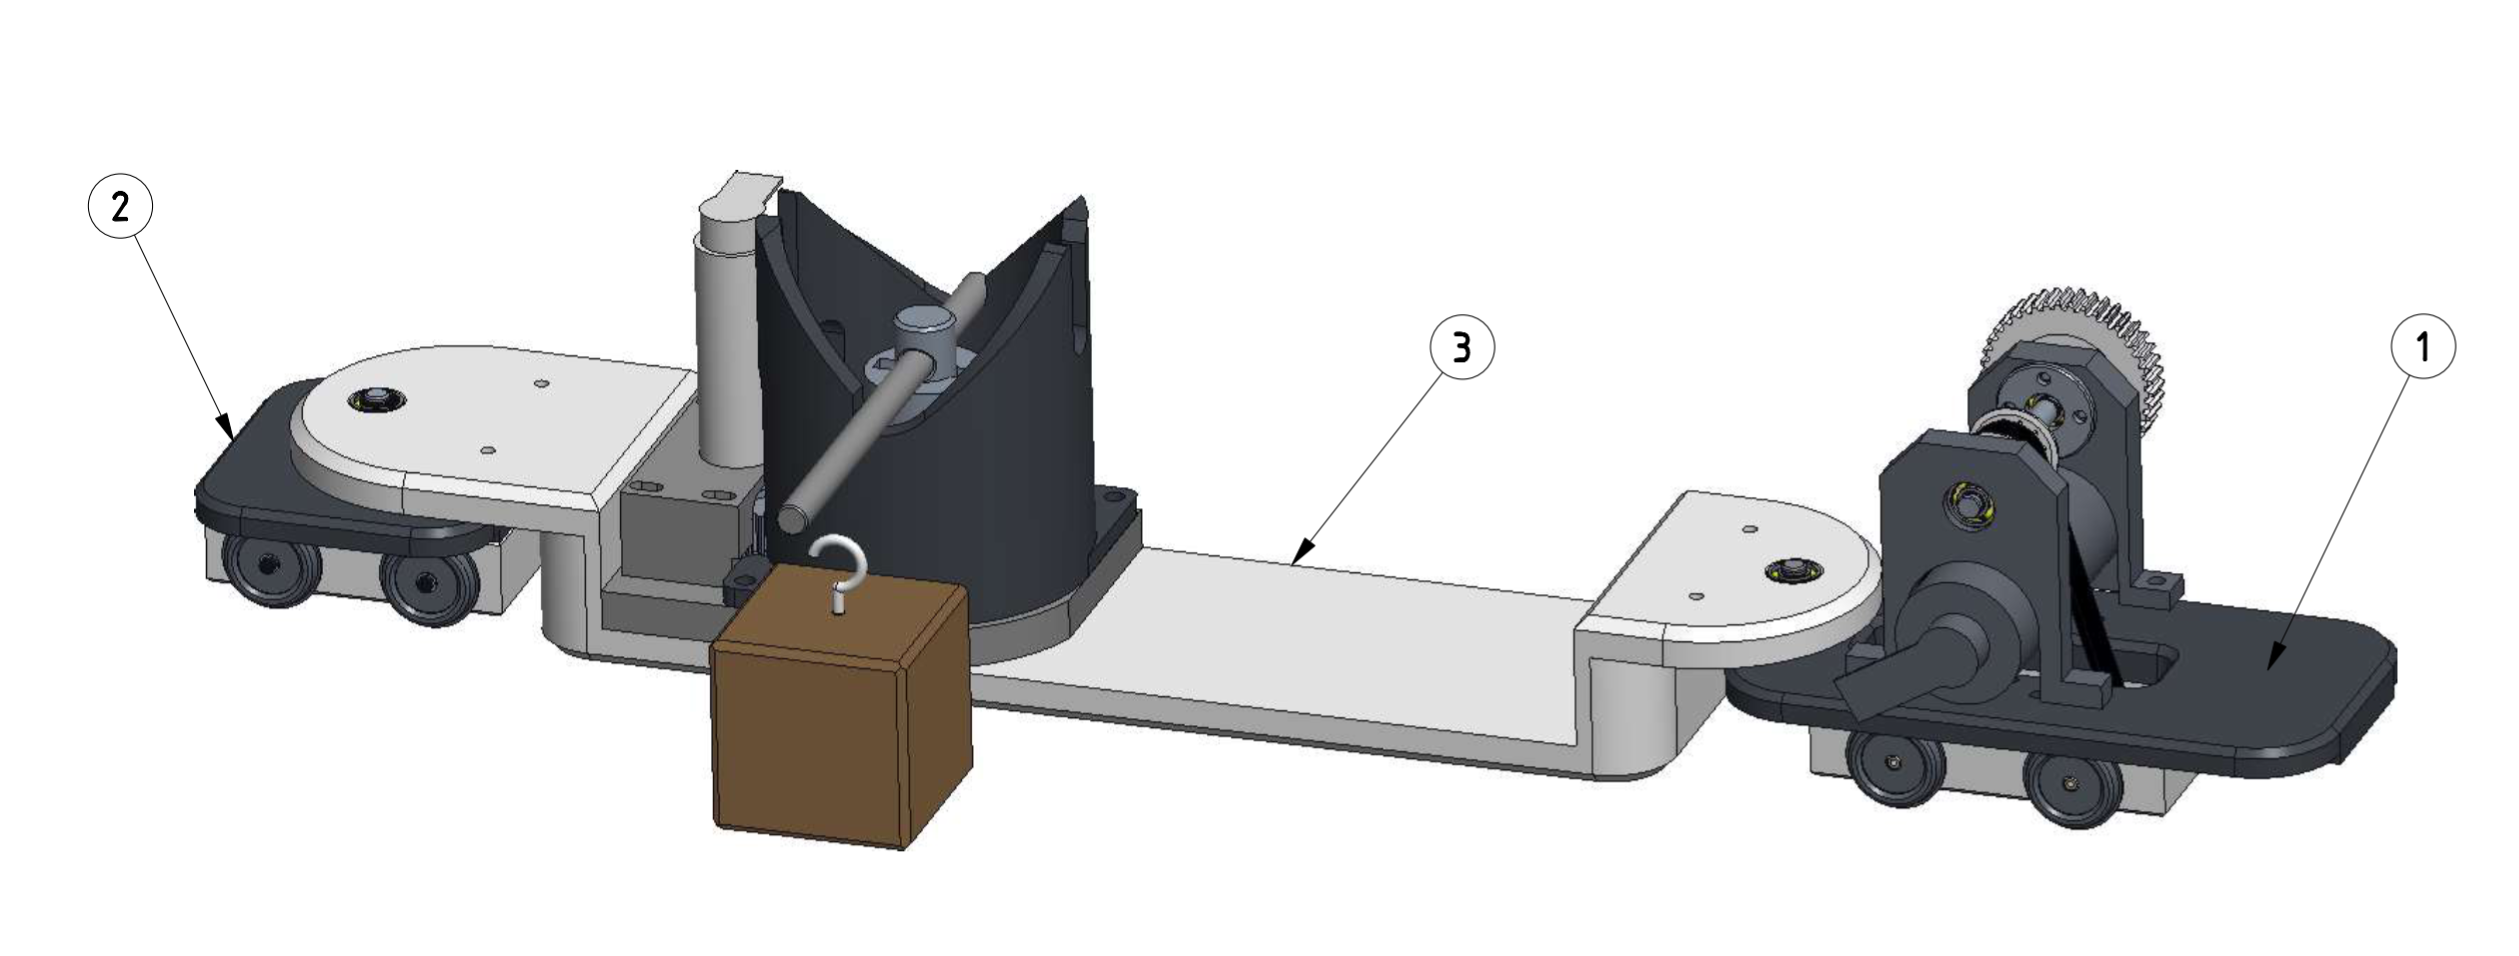
\includegraphics[width=0.9\textwidth]{Lokomotive.png}
        \caption{Baugruppe Lokomotive}
        \label{fig:bg_lokomotive}
    \end{figure}

    \begin{table}[H] \centering
        \begin{tabular}{|l|l|}
        \hline
        \textbf{Position} & \textbf{Bezeichnung}\\
        \hline
        Position 1          & Antriebswagen\\
         \hline
        Position 2          & Führungswagen\\
        \hline
        Position 3          & Ladungsträger\\
        \hline
        \end{tabular}
        
        \caption{Positionsnummern der Lokomotive mit Bezeichnungen}
        \label{tab:com_tiny_pi}
        \end{table}
    
    In der Querschnittsdarstellung in Abbildung \ref{fig:schnitt_lokomotive} die Lagerungen zwischen dem Ladungsträger und dem Antriebswagen beziehungsweise dem Führungswagen sowie die Antriebseinheit besser sichtbar. Der Aufbau der Unterbaugruppen wird in den nächsten Abschnitten vorgestellt.
   
    \begin{figure}[H] %Lokomotive im Schnitt
        \centering
        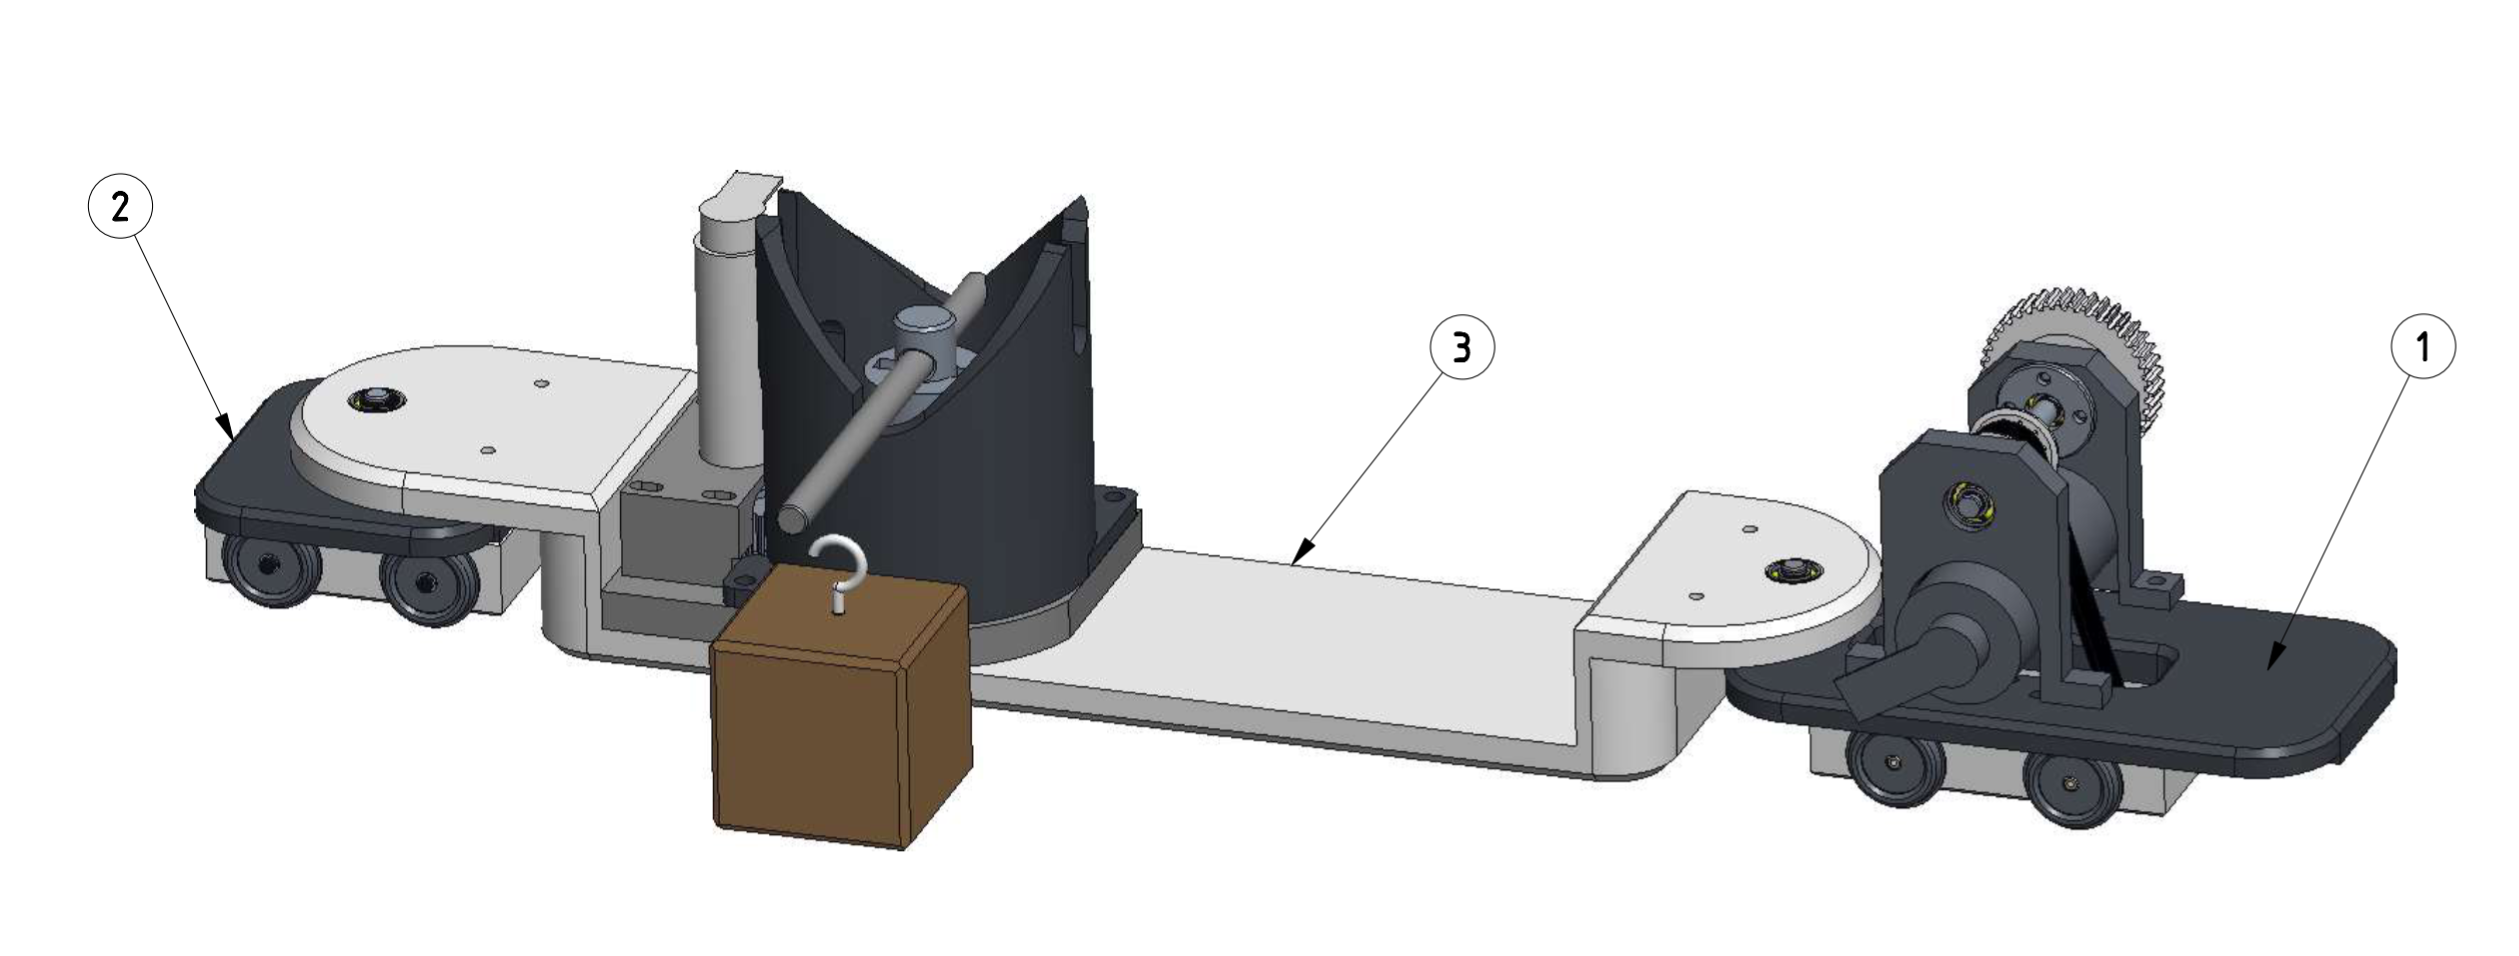
\includegraphics[width=0.9\textwidth]{Lokomotive.png}
        \caption{Schnittansicht der Lokomotivenbaugruppe}
        \label{fig:schnitt_lokomotive}
    \end{figure}
    \newpage

    \subsubsection{Antriebswagen}
    Der Grundaufbau der beiden Wägen ist derselbe, mit dem Unterschied, dass der Antriebswagen durch einen Motor angetrieben wird. Der Grundwagen beziehungsweise der Führungswagen in Abbildung besteht aus einem Rahmen und einer Platte, welche miteinander verstiftet (Position 2) und verschraubt (Position 3) sind. Im Rahmen werden die beiden Achsen jeweils mit einem Los- und einem Festlager lagert. Die Achsen sind an beiden Enden mit einem Gewinde versehen, damit die Räder bei Bedarf schnell und einfach gewechselt werden können, ohne dass der ganze Wagen auseinander genommen werden muss. Die Anfräsfläche auf der Welle (Position 5) dient für das bessere Befestigen der Räder durch einen Gabelschlüssel.

     \begin{figure}[H] %Führungswagen
        \centering
        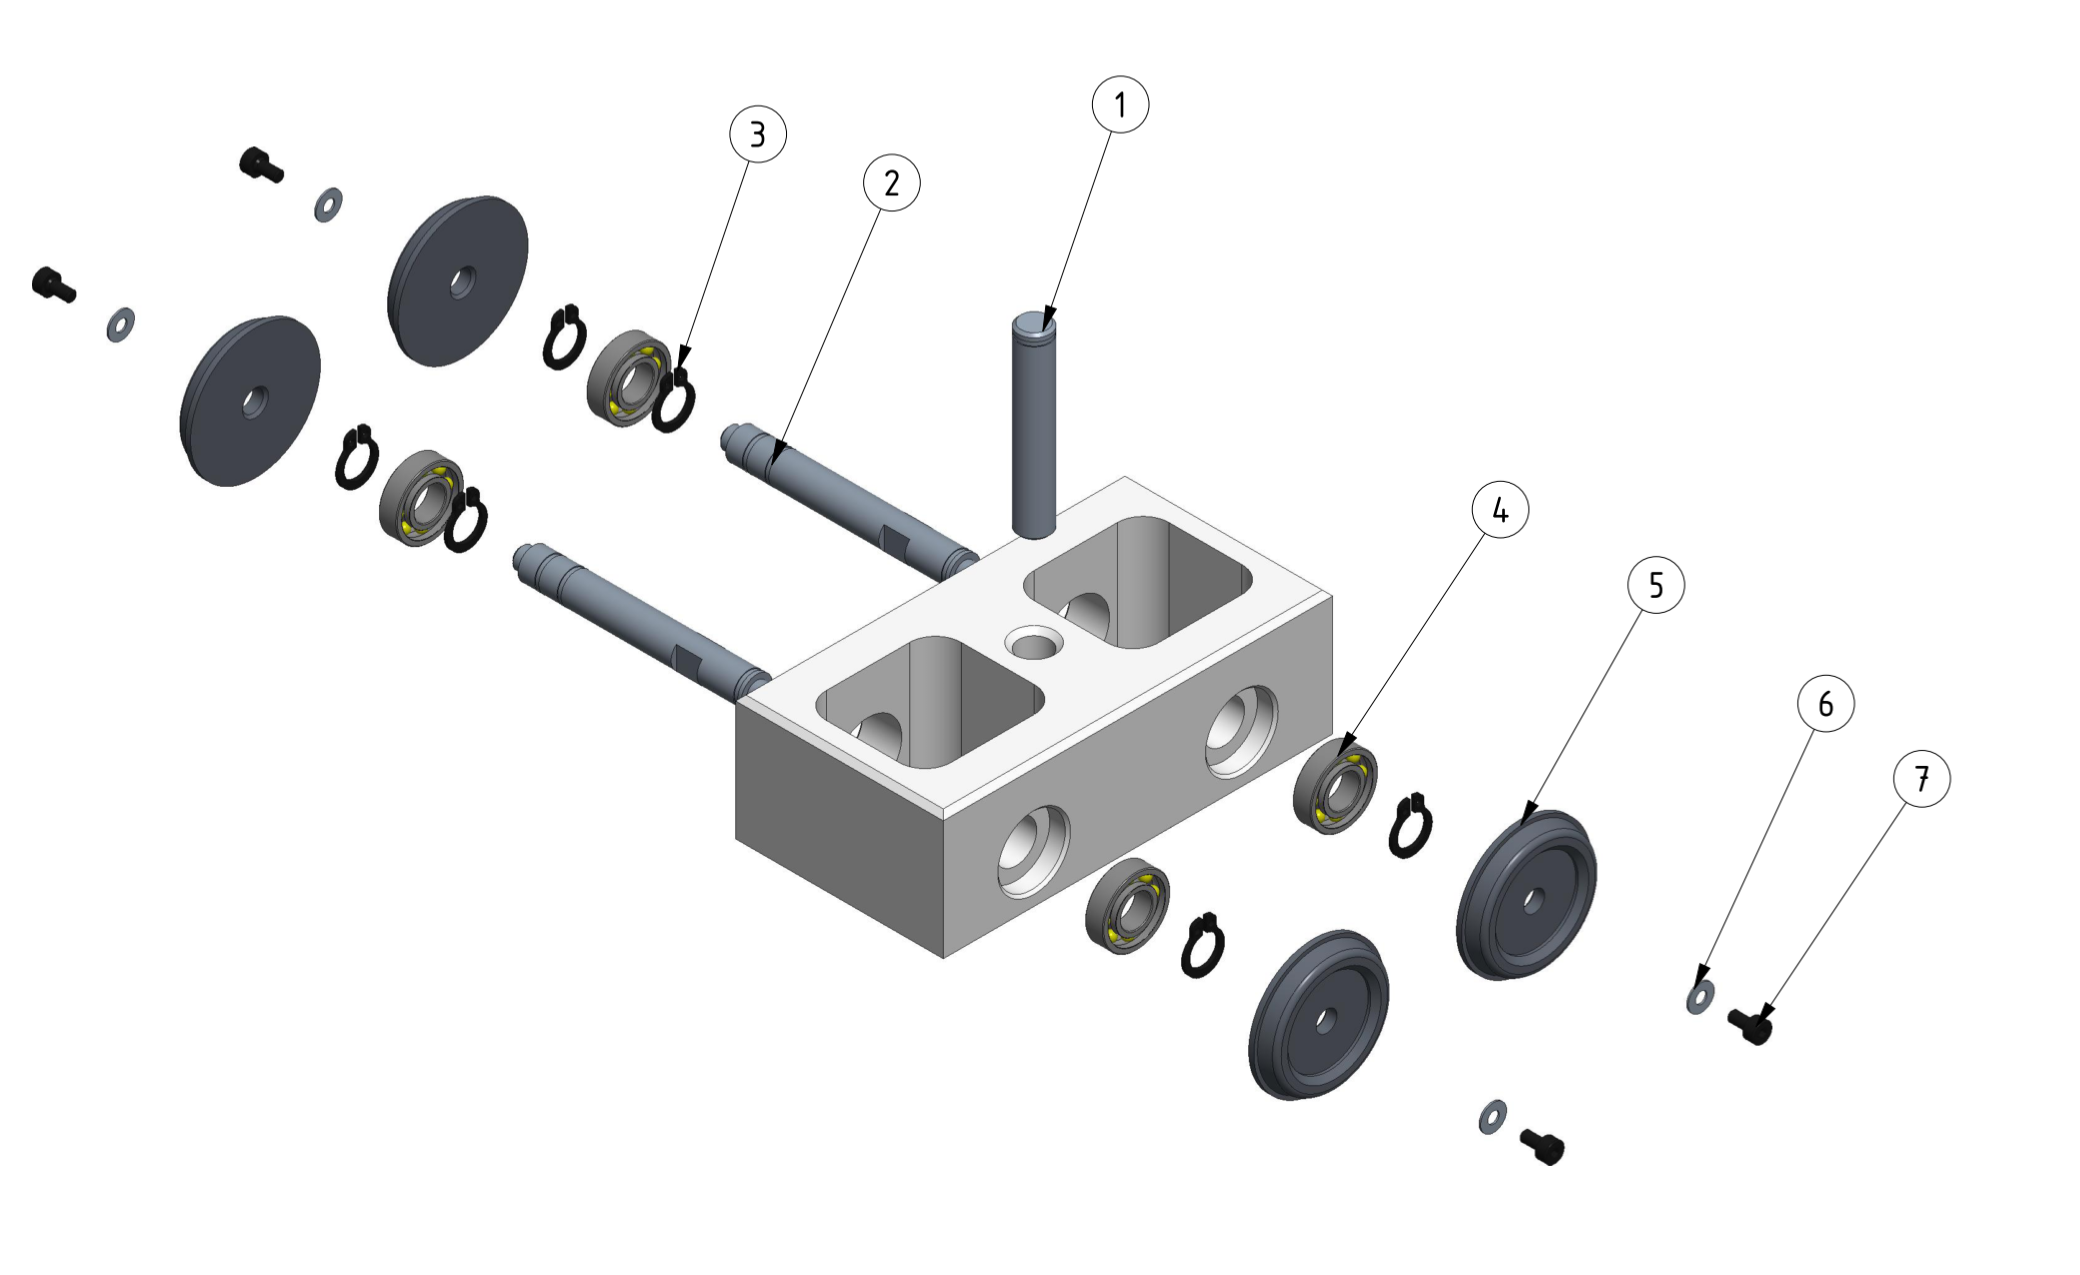
\includegraphics[width=0.9\textwidth]{Fuehrungswagen.png}
        \caption{Explosionsdarstellung Führungswagen}
        \label{fig:expl_fuehrungswagen}
    \end{figure}   

    \begin{table}[H] \centering
        \begin{tabular}{|l|l|}
        \hline
        \textbf{Position} & \textbf{Bezeichnung}\\
        \hline
        Position 1          & Drehachse Wagen-Ladungsträger\\
         \hline
        Position 2          & Stife für das Verstiften von Rahmen und Platte\\
        \hline
        Position 3          & Zylinderschrauben für das Befestigen der Platte am Rahmen\\
        \hline
        Position 4          & Platte\\
        \hline
        Position 5          & Achsen mit Gewinden an beiden Enden und Anfräsfläche für Gabelschlüssel\\
        \hline
        Position 6          & Sicherungsring für Rillenkugellager\\
        \hline
        Position 7          & Rillenkugellager (Loslager)\\
        \hline
        Position 8          & Eingepresstes Rillenkugellager (Festlager)\\
        \hline
        Position 9          & Rad\\
        \hline
        Position 10         & Unterlagscheibe\\
        \hline
        Position 11         & Zylinderschraube\\
        \hline
        \end{tabular}
        
        \caption{Kommunikation Frames: Tiny $\Rightarrow$ Pi}
        \label{tab:com_tiny_pi}
        \end{table}
    \newpage
    Der Antriebswagen in Abbildung ist grundsätzlich gleich aufgebaut wie der Führungswagen, jedoch ist der Rahmen aufgrund des Riemenantriebs etwas anders Aufgebaut. Die Platte, welche auf dem Rahmen angebracht ist, wurde für die Kameras für die Signal- und Spurerkennung grösser dimensioniert. Die Kamera für die Spurerkennung wird einstellbar befestigt, damit bei der Testphase des Prototyps Optimierungen vorgenommen werden können. Die Stromübetrag von der Shiene auf die Lokomotive erfolgt über vier Schleifkontakte. Davon sind jeweils zwei ein einem Wagen zwischen den Rädern angebracht.

    \begin{figure}[H] %Antriebswagen
        \centering
        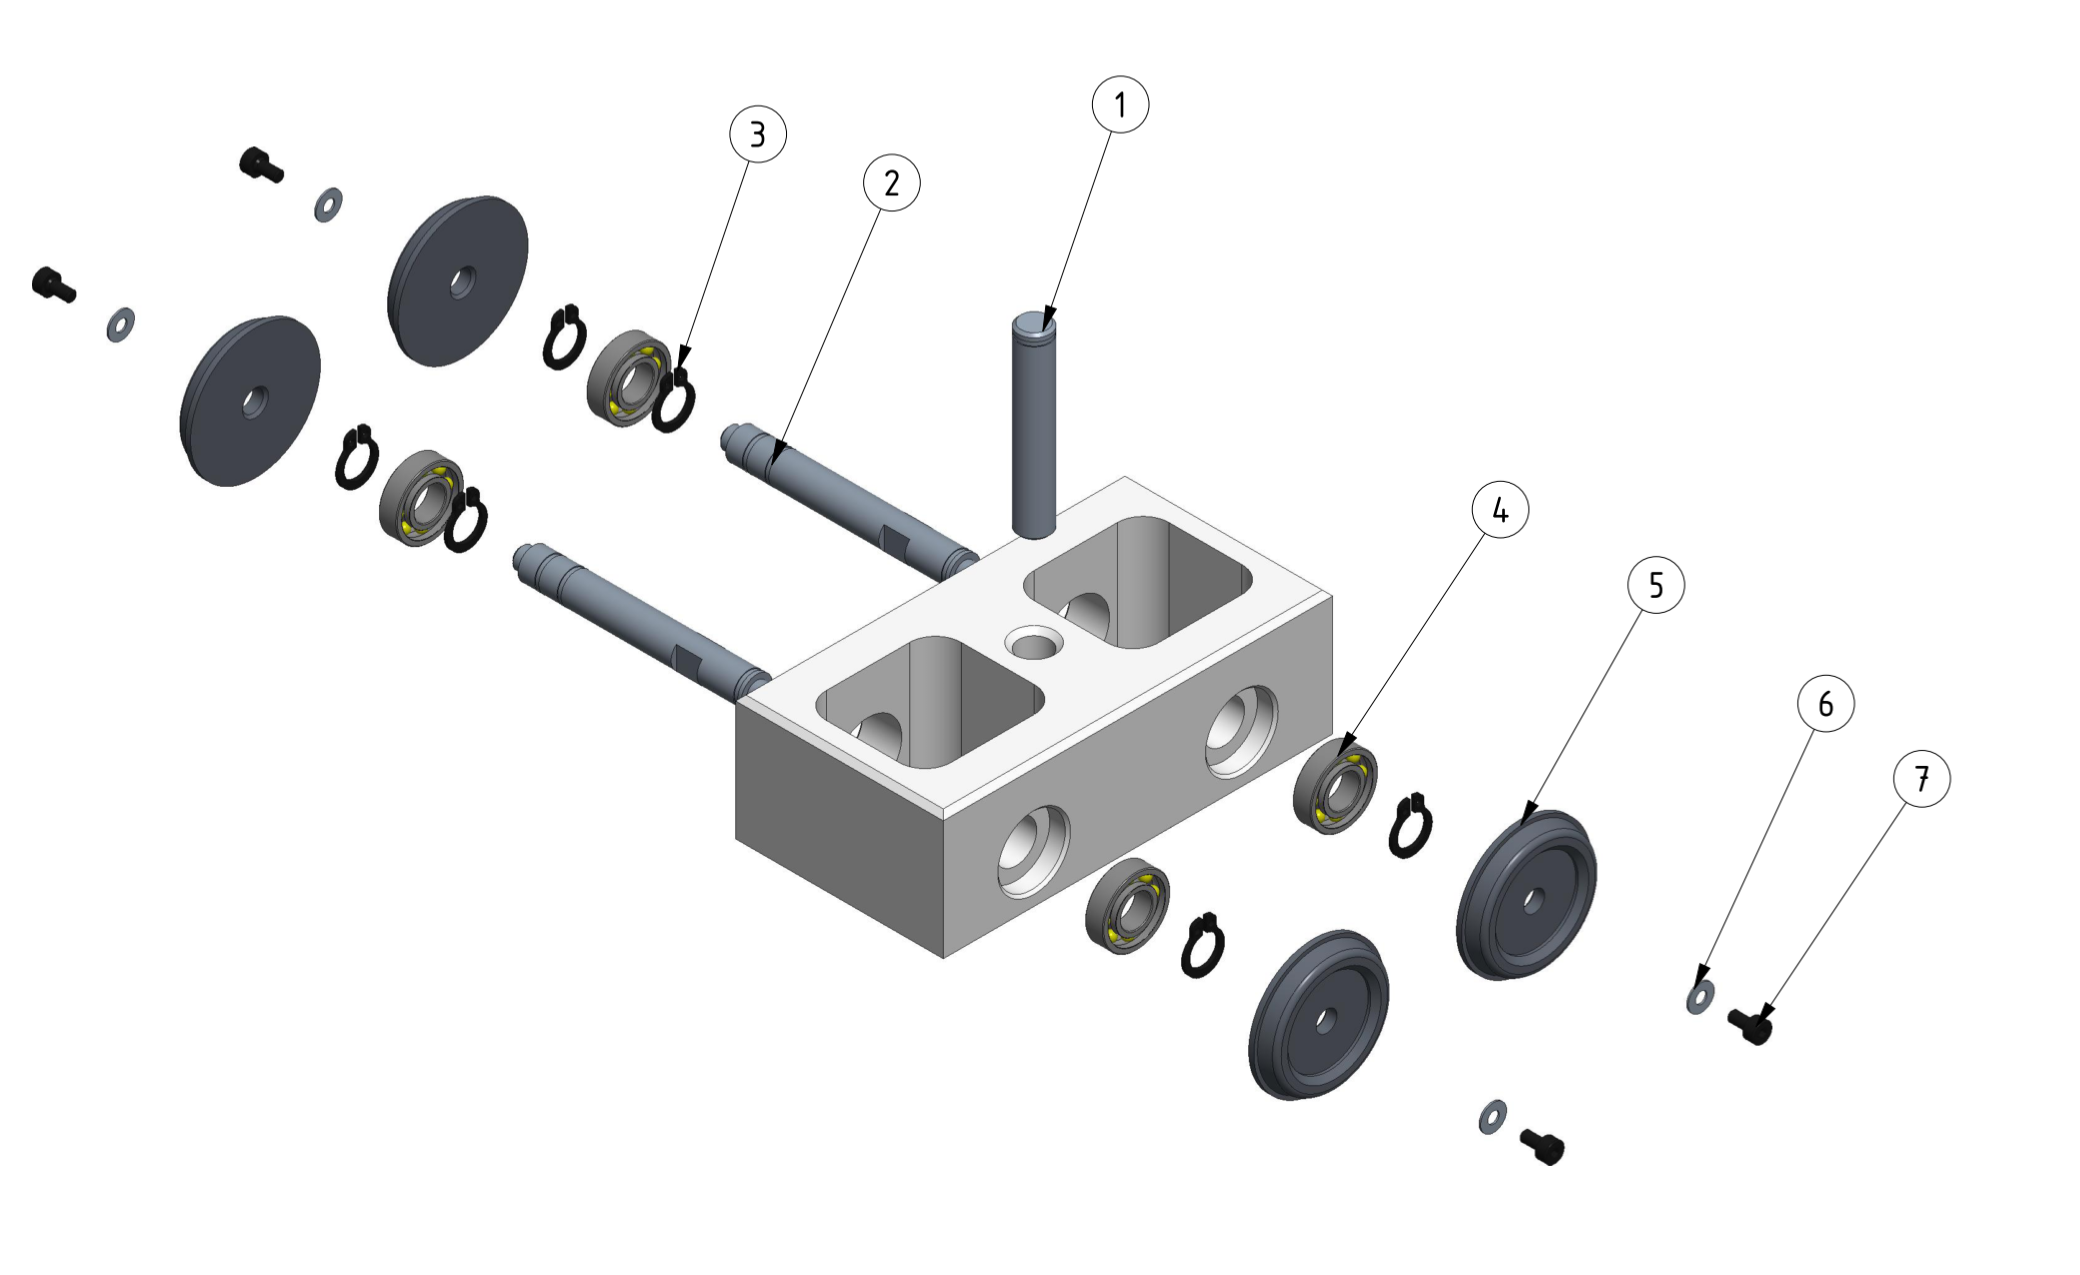
\includegraphics[width=0.9\textwidth]{Fuehrungswagen.png}
        \caption{Baugruppe Antriebswagen}
        \label{fig:Antriebswagen}
    \end{figure} 

    \begin{table}[H] \centering
        \begin{tabular}{|l|l|}
        \hline
        \textbf{Position} & \textbf{Bezeichnung}\\
        \hline
        Position 1          & Wagen\\
         \hline
        Position 2          & Antriebseinheit\\
        \hline
    \end{tabular}
    
    \caption{Kommunikation Frames: Tiny $\Rightarrow$ Pi}
    \label{tab:com_tiny_pi}
    \end{table}

    Antriebseinheit in Abbildung besteht aus einem Grundgestell, an welchem die Lagerung der Antriebswelle und der Motor angebracht sind. Das Drehmoment vom Motor wird über ein geradverzahntes Zahnrad mit einem Übersetzungsverhältnis von 1:2 auf eine Achse übertragen. Von dieser wird es über einen Riemen auf die beiden Radachsen und somit auf die Räder weitergeleitet. Durch die Berechnung der maximalen Geschwindigkeit wird entsprechend der Motor ausgelegt, was im nächsten Abschnitt genauer beschrieben wird.

    \begin{figure}[H] %Antriebseinheit
        \centering
        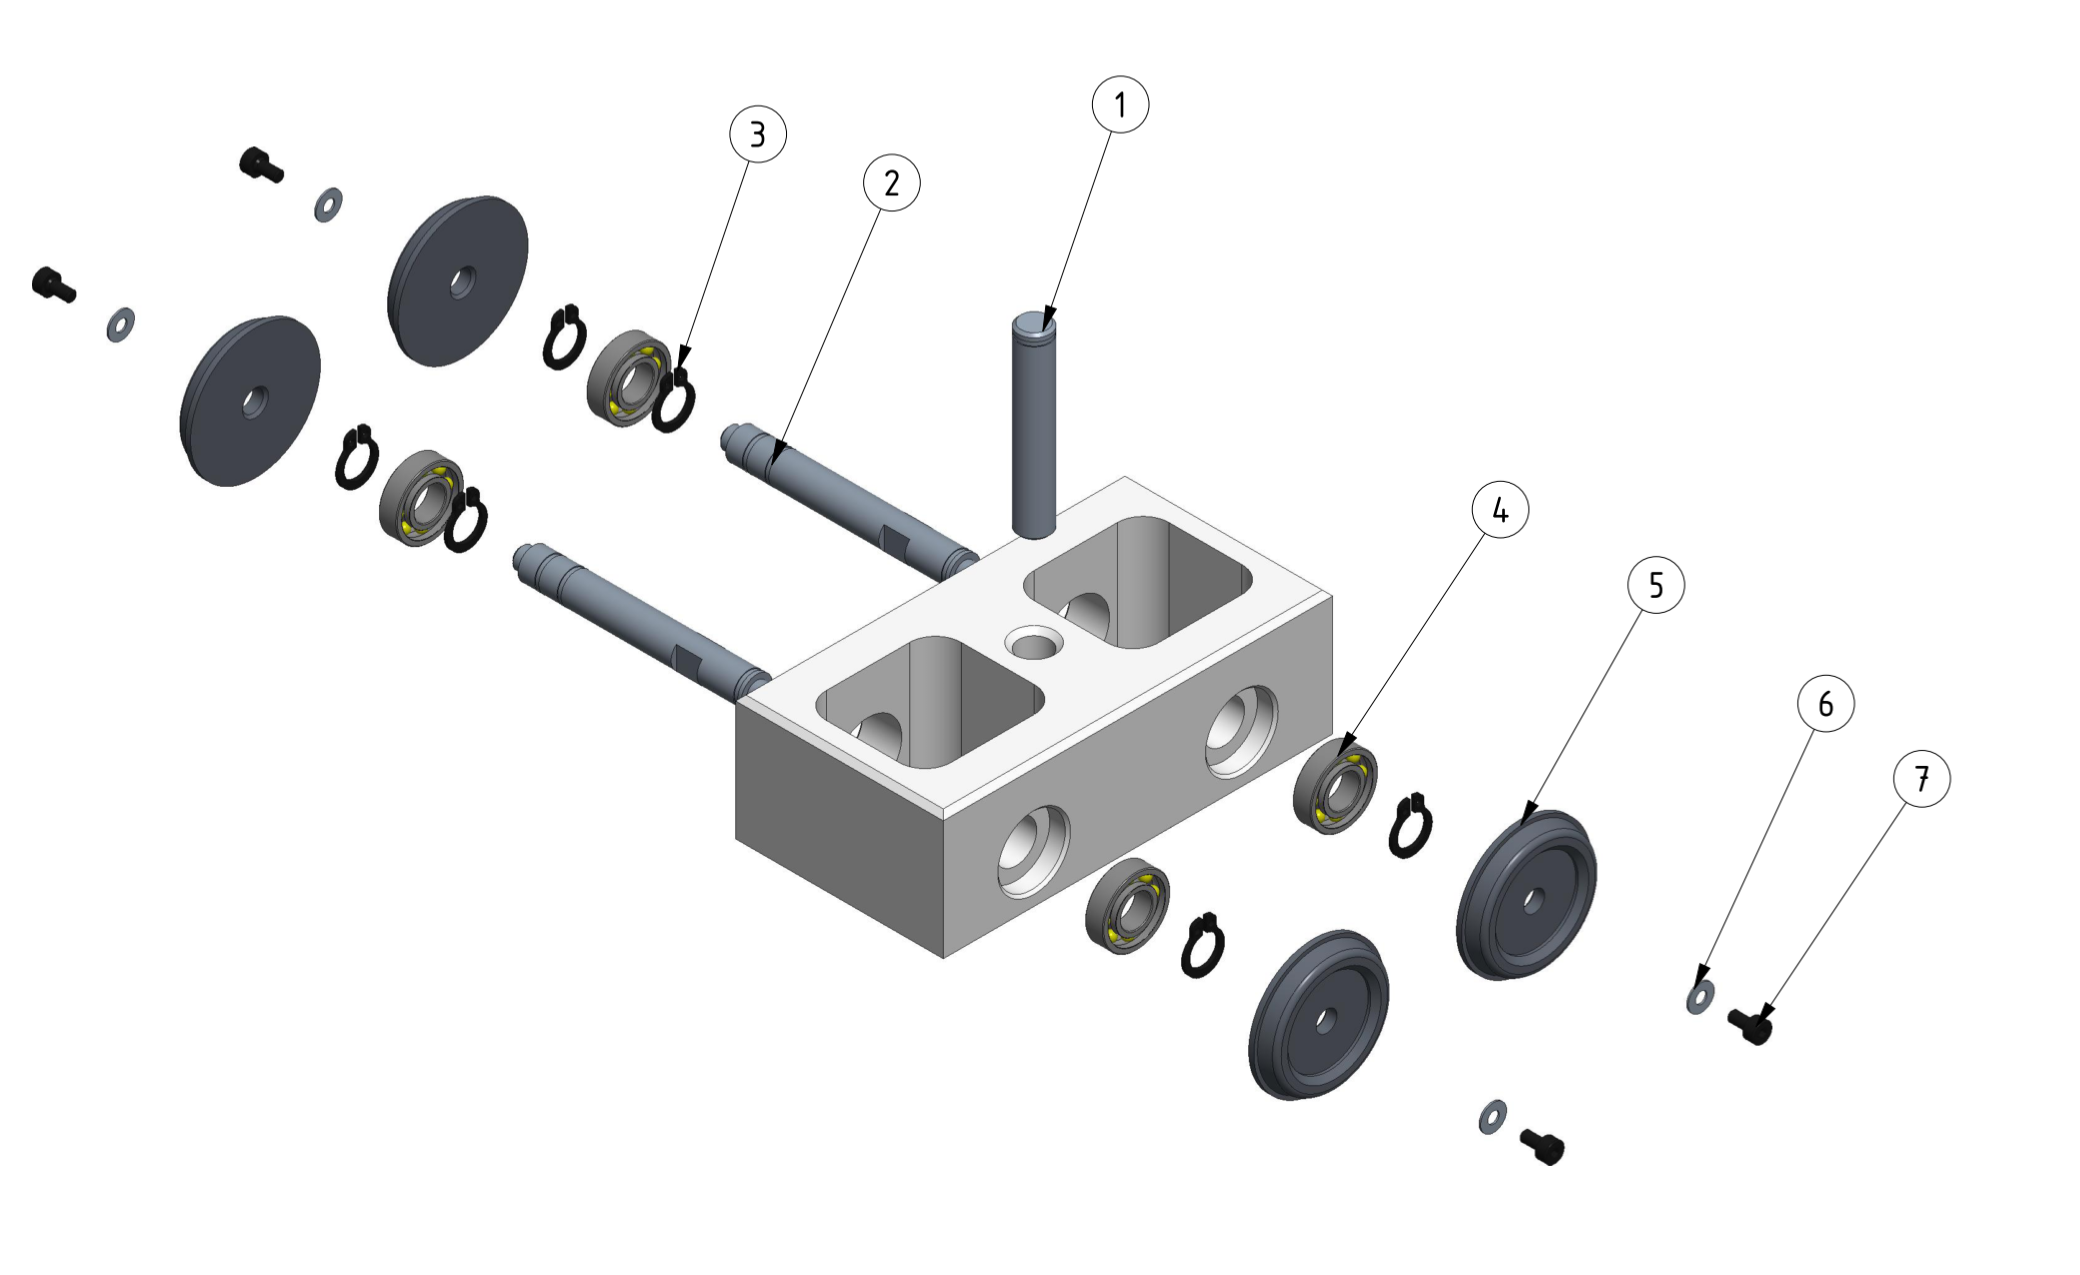
\includegraphics[width=0.9\textwidth]{Fuehrungswagen.png}
        \caption{Explosionsdarstellung Führungswagen}
        \label{fig:antriebseinheit}
    \end{figure} 

    \begin{table}[H] \centering
        \begin{tabular}{|l|l|}
        \hline
        \textbf{Position} & \textbf{Bezeichnung}\\
        \hline
        Position 1          & Drehachse Wagen-Ladungsträger\\
         \hline
        Position 2          & Stife für das Verstiften von Rahmen und Platte\\
        \hline
        Position 3          & Zylinderschrauben für das Befestigen der Platte am Rahmen\\
        \hline
        Position 4          & Platte\\
        \hline
        Position 5          & Achsen mit Gewinden an beiden Enden und Anfräsfläche für Gabelschlüssel\\
        \hline
        Position 6          & Sicherungsring für Rillenkugellager\\
        \hline
        Position 7          & Rillenkugellager (Loslager)\\
        \hline
        Position 8          & Eingepresstes Rillenkugellager (Festlager)\\
        \hline
        Position 9          & Rad\\
        \hline
        Position 10         & Unterlagscheibe\\
        \hline
        Position 11         & Zylinderschraube\\
        \hline
        \end{tabular}
        
        \caption{Kommunikation Frames: Tiny $\Rightarrow$ Pi}
        \label{tab:com_tiny_pi}
        \end{table}
    \newpage

    \textbf{Beschleunigungsberechnung}\\
    Wie schnell die Lokomotive beschleunigen kann hängt von der Reibung zwischen Rad und schiene und der Masse des Zuges ab. Die Grunddefinition der Beschleunigung ist der Quotient von Kraft und Masse. Die Reibung ist durch den Reibkoeffizienten bestimmt, welcher sich je nach Materialpaarung 

    Die Kraft für das aus dem Stillstand in Fahrt zu bringende ist am grösste. Anschliessend wird die Reibung kleiner (Da rollreibung).

    \begin{table}[H] \centering
        \begin{tabular}{|l|l|l|}
        \hline
        \textbf{Material Schiene} & \textbf{Material Rad} & \textbf{Reibungskoeffizient}\\
        \hline
        Stahl                                & Stahl        & 0.02\\
         \hline
        Stahl                                & Holz         & 0.02\\
        \hline
        Stahl                                & Kunststoff   & 0.02\\
        \hline
        Stahl                                & Gummi        & 0.02\\
        \hline
        \end{tabular}\\
        
        \caption{Reibungskoeffizienten verschiedener Materialpaarungen}
        \label{tab:com_tiny_pi}
        \end{table}
    
    Um die maximale Beschleunigung zu berechnen, wird das Gesamtgewicht der Lokomotive auf die vier Räder aufgeteilt. In der Tabelle \ref{tab:groessen_beschleunigung} sind die gegeben Grössen für die nachfolgenden Berechnungen aufgelistet.

    \begin{table}[H] \centering
        \begin{tabular}{|l|l|}
        \hline
        \textbf{Grösse} & \textbf{Wert}\\
        \hline
        Durchmesser Rad [D]          & 30 Milimeter\\
         \hline
        Reibungskoeffizient [k]      & 0.3\\
        \hline
        \end{tabular}
        
        \caption{Grössen für die Beschleunigungsberechnung}
        \label{tab:groessen_beschleunigung}
        \end{table}   

    F\textsubscript{Rad}=\(\frac{F\textsubscript{G}}{8}\)=\(\frac{m*g=3kg*9.81m/s^2}{8}\)=0.375\\

    F\textsubscript{Reibung}=\(F\textsubscript{Rad}*k\)=\(0.375N*0.3=29.4N\)=0.1125N\\

    M\textsubscript{Rad}=\(F\textsubscript{Rad}*2*D\textsubscript{Rad}\)=\(\frac{m*g=3kg*9.81m/s^2}{8}\)=0.375Nm\\

    a\textsubscript{max}=\(\frac{F\textsubscript{Reibung}}{\frac{F\textsubscript{Rad}}{g}}\)=\(\frac{F\textsubscript{Reibung}}{\frac{F\textsubscript{Rad}}{g}}\)\\

    \textbf{Geschwindigkeitsberechnung}\\
    Die Fahrgeschwindigkeit der Lokomotive wird durch drei Faktoren bestimmt. Einerseits muss die maximale Geschwindigkeit der Anforderungsliste eingehalten werden und andererseits wird die Geschwindigkeit in der Kurvenfahrt durch den Schwerpunkt des Fahrzeuges und durch die maximale Haftreibkraft zwischen Schiene und Rad eingeschränkt.

    In der Anforderungsliste wurde eine minimale Geschwindigkeit von 0.5 Meter pro Sekunde festgelegt. Der begrenzende Faktor der Geschwindigkeit in der Kurve ist der Schwerpunkt der Lokomotive. Je tiefer dieser ist, umso schneller kann die Kurve abgefahren werden. Über die Zentripedalkraft und die Gewichtskraft der Lokomotive wird die Momentengleichung aufgestellt. 

    \begin{table}[H] \centering
        \begin{tabular}{|l|l|}
        \hline
        \textbf{Grösse} & \textbf{Wert}\\
        \hline
        Minimaler Radius  [r]                               & 0.8 Meter\\
         \hline
        Masse [m]                                           & 3 Kilogramm\\
        \hline
        Schwerpunkt in x-Achse (maximaler Wert) [x]         & Meter\\
        \hline
        Schwerpunkt in y-Achse (maximaler Wert) [y]         & Meter\\
        \hline
        \end{tabular}\\
        
        \caption{Kommunikation Frames: Tiny $\Rightarrow$ Pi}
        \label{tab:com_tiny_pi}
        \end{table}

        Die Zentripedalkraft und die Gewichtskraft sind wie folgt definiert:\\
    
    F\textsubscript{G}=\(m*g=3kg*9.81m/s^2=29.4N\)\\

    F\textsubscript{max z}=\(\frac{m*v^2}{r}\)=\(\frac{m*v^2}{r}\)\\
    
    Da das Drehmoment eine vektorielle Grösse ist, müssen die beiden entstehenden Momente am Drehpunkt "P" auf am Gleis zusammen Null ergeben beziehungsweise gleich gross sein, damit es "statisch" bestimmt ist. Die Berechnungen sind auf den kleinsten Kurvenradius ausgelegt, da dort die grössere Zentripedalkraft entsteht.\\

    F\textsubscript{max z}=\(\frac{F\textsubscript{G}*x+F\textsubscript{A}*a}{y}\)=\(\frac{F\textsubscript{G}*x+F\textsubscript{A}*a}{y}\)\\

    %Bild von Zug (Ansicht von vorne) mit Schwerpunkt und Positionsnummern
    
    Das Kippmoment wird durch den Aufbau der Lokomotive minimiert. Da der Schwerpunkt durch die beiden Wagen mehr in das Zentrum des Kreismittelpunktes rückt.
    
    Um möglichst viel Drehmoment auf das Rad zu übertragen, muss die Haftreibung maximiert werden, da die Beschleunigung davon abhängt. Die Reibungskoeffizienten wurden experimentell ermittelt. Dazu wurden verscheidene Materialen auf das Gleis gelegt und mit einer Federwage die Reibungskraft ermittelt. Der Versuch wurde mit den Materialien Kunstoff, Holz, Stahl und Gummi ausgeführt.

    \textbf{Motorauslegung}\\
    %Text von Schöni

    \subsubsection{Ladungsträger}
    Der Ladungsträger ist das Verbindungselement von Antriebswagen und Führungswagen. Er wird an beiden Enden drehbar mit Radialkugellager gelagert.

    Der Träger besteht aus drei Teilen (siehe Abbidlung). Der Hauptgrund ist die einfachere und kostengünstigere Herstellung.

    %Berechnung Kugellagerkräfte

    \begin{figure}[H] %Ladungsträger
        \centering
        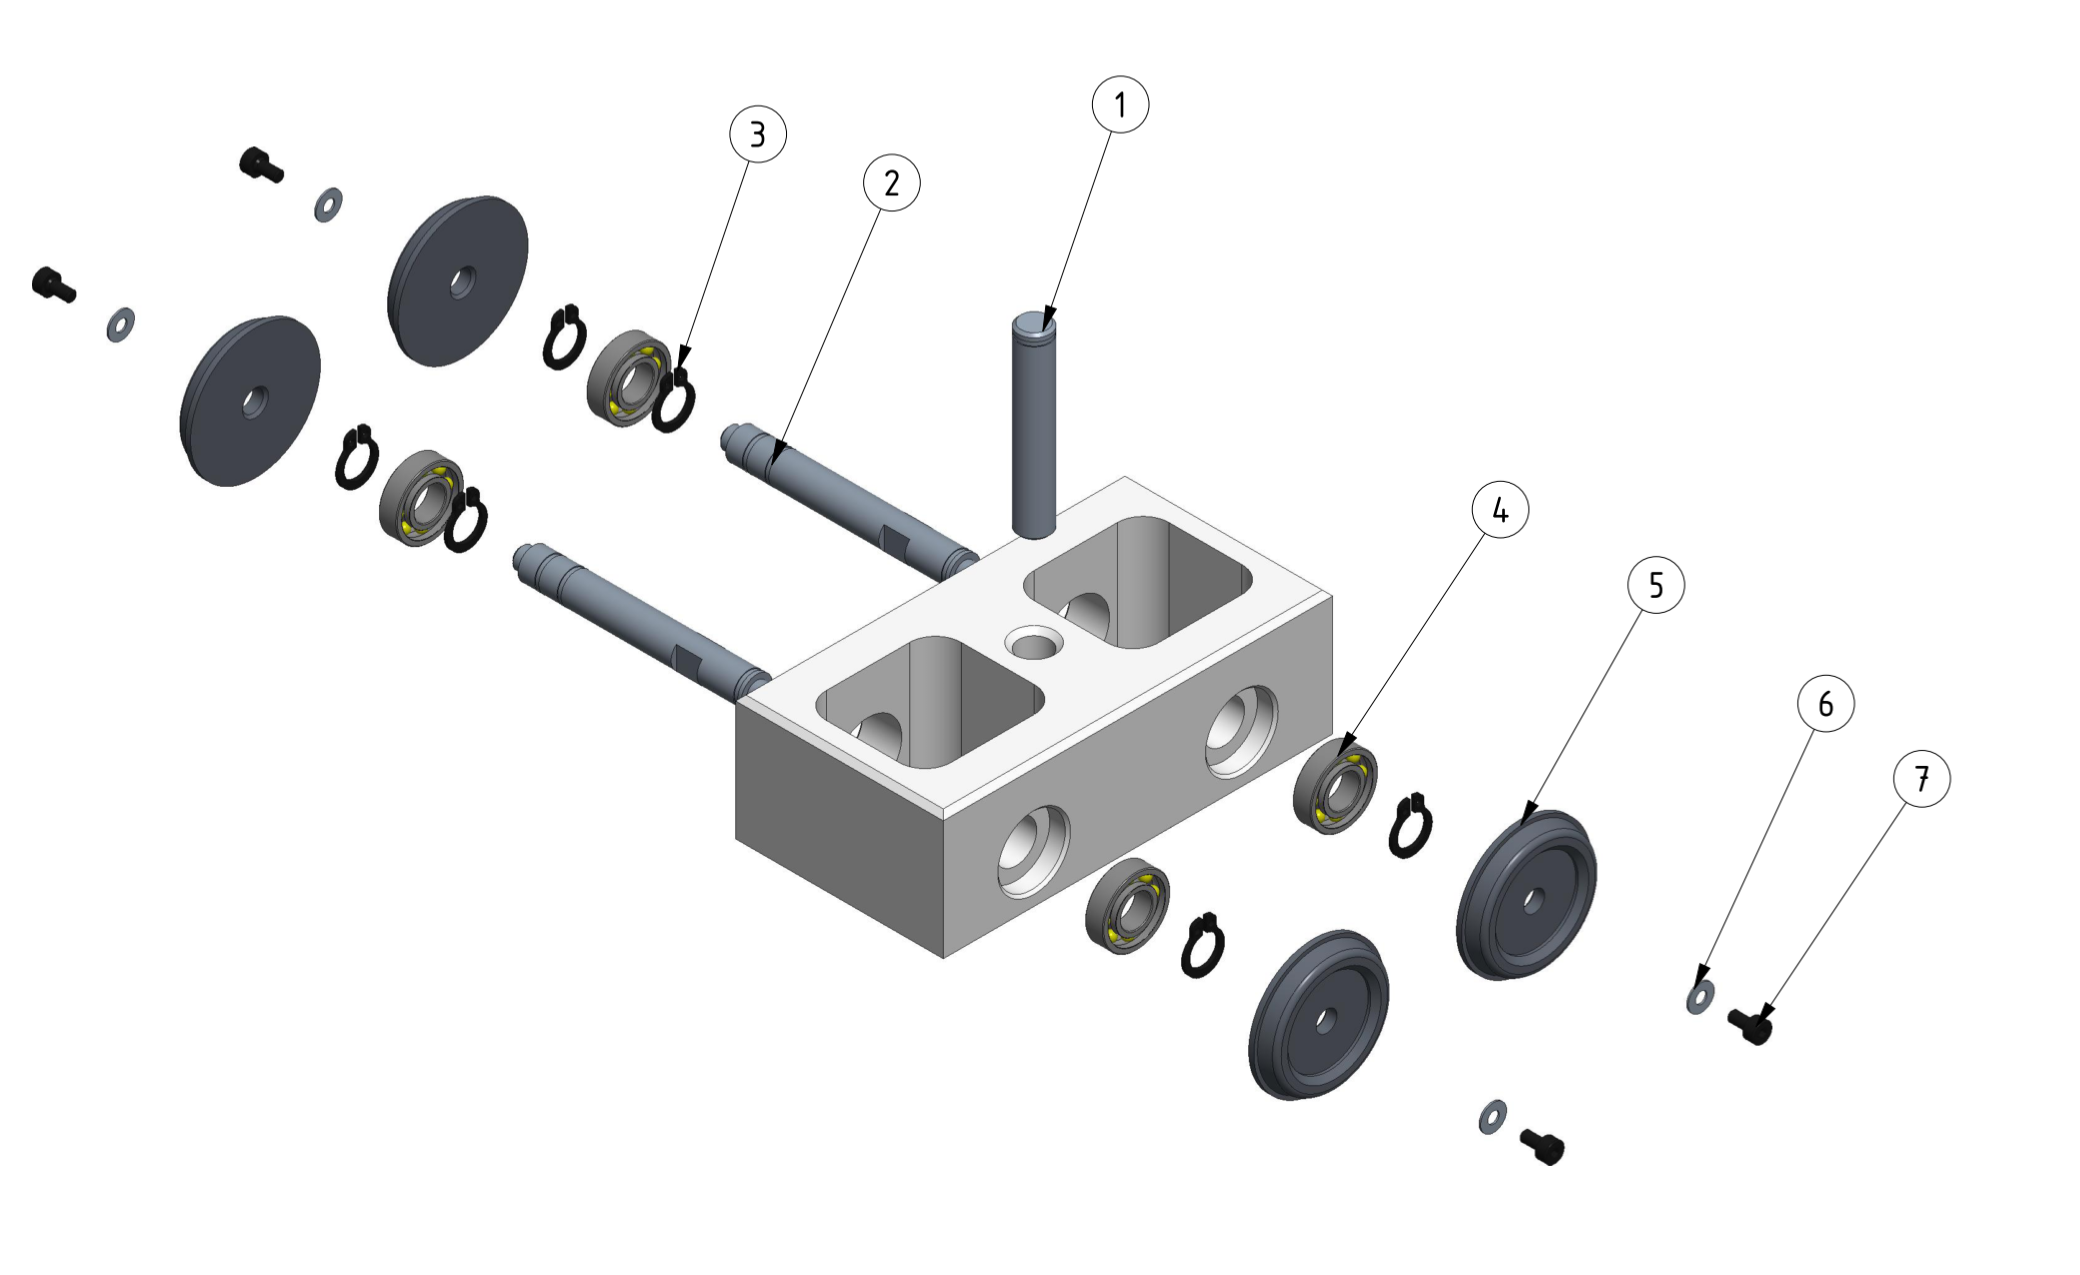
\includegraphics[width=0.9\textwidth]{Fuehrungswagen.png}
        \caption{Explosionsdarstellung Führungswagen}
        \label{fig:expl_fuehrungswagen}
<<<<<<< HEAD
    \end{figure}\\
=======
    \end{figure}
>>>>>>> feature/Funktionsbeschrieb_fortfahren

    \begin{table}[H] \centering
        \begin{tabular}{|l|l|}
        \hline
        \textbf{Position} & \textbf{Bezeichnung}\\
        \hline
        Position 1          & Drehachse Wagen-Ladungsträger\\
         \hline
        Position 2          & Stife für das Verstiften von Rahmen und Platte\\
        \hline
        Position 3          & Zylinderschrauben für das Befestigen der Platte am Rahmen\\
        \hline
        Position 4          & Platte\\
        \hline
        Position 5          & Achsen mit Gewinden an beiden Enden und Anfräsfläche für Gabelschlüssel\\
        \hline
        \end{tabular}
        
        \caption{Kommunikation Frames: Tiny $\Rightarrow$ Pi}
        \label{tab:com_tiny_pi}
        \end{table}

    \textbf{Würfeltransport}\\
    Um den Würfel rechts neben der Gleisstrecke aufzunehmen wird eine steuerungstechnisch sowie mechanisch einfache Lösung angestrebt. Wie aus dem morphologischen Kasten (Anhang) und der Nutzwertanalyse hervor geht, wird die Würfelaufnahme mittels eines Drahts und einem Stab durchgeführt. Damit nur ein Aktor angesteuert werden muss wird von dem Prinzip einer Kurvenscheibe Gebrauch gemacht.  Die gesamte Vorrichtung besteht grundsätzlich aus drei Elementen. Einem Kran zur Lastaufnahme, einem Antriebsstrang und der Kurvenscheibe.

    Der Kran besteht aus drei Drehteilen, welche mit einer Pressverbindung zusammengefügt wurden. Der Grundkörper des Krans wird auf Grund seiner optimalen Gleiteigenschaften und der geringen Dichte aus Teflon gefertigt. Der kleinere Stahlstift ist für die Drehmomentübertragung zuständig. Der Grössere der beiden Stahlstifte ist der eigentliche Ausleger. An dessen ende wird ein Draht aus Federstahl geformt und angehängt. Dieser Draht soll als Haken zur Lastaufnahme dienen. Weiter ist der Ausleger in beide Richtungen von der Drehachse ausgedehnt, da die Kurvenscheibe zwei Laufflächen hat, um für einen stabilen Hub zu sorgen. Der ganze Aufbau wird mittels einer Spielpassung in einer Bohrung mit zwei längsnuten in einem 3D gedruckten, modifizierten Zahnrad gelagert.

    Der Antrieb besteht aus einem Motor, dessen Aufhängung und zwei Zahnrädern. Der Motor ist ein bürstenbehafteter Motor mit Encoder und Getriebe vornedrauf. Mit dieser Variante und der Übersetzung von Getriebe und den Zahnrädern kann von der Steuerung aus genau definiert werden, wie viele Umdrehungen der Motor benötigt, um mit dem Kranausleger eine Viertelumdrehung zu fahren. Das eine Zahnrad ist Standard und von Mädler eingekauft. Das zweite Zahnrad jedoch wurde nur als STEP von Mädler heruntergeladen und anschliessend im CAD bearbeitet. Die Bohrung und der Flansch in der Mitte wurden verlängert und mit zwei Längsnuten versehen. Die Bohrung gilt als Axialführung und die Nuten als Drehmomentübertragung.

    Die Kurvenscheibe ist ebenfalls ein 3D-Druckteil. Der Grundkörper ist ein Rohr mit dem Aussendurchmesser 80 mm. An diesem wurden zwei Bahnführungen mittels Freiformflächen für den Kranausleger erzeugt. Die Steigung dieser Flächen ist variabel. Zu Beginn ist die Steigung gering und wird dann exponentiell grösser. Dies wurde aus dem einen Grund gewählt, damit das Anfahren für den Motor nicht zu streng ist. Nachdem die Drehbewegung und der vertikale Hub gemacht wurden, stoppt der Motor und der Kranausleger sollte durch die Schwerkraft heruntergezogen werden. Der Würfel wird nun in der für ihn vorgesehenen Aufnahme auf dem Zug platziert.

\end{document}